\subsection{k-medoids clustering}

\qquad The \textit{k-medoids} clustering method is similar to \textit{k-means}, except that the former takes $k$ data points as centers while the latter makes use of means from $k$ disjoint sets. The \textit{k-medoids} algorithm first picks up k data points randomly, and assign other points to their nearest centers, thus forming k clusters. Within each cluster, select the data point which minimizes the sum of the distances  between it and other points. Repeat the previous steps until convergence. Our \textit{k-medoids} clustering is based on the data of county level because for individual level there will be too many samples for the algorithm to work. Instead of using \textit{Gap} statistics and \textit{Silhouette} plot, this we mainly rely on visualization to determine the number of clusters because both the former methods tend to be conservative \textbf{[ref!]} and the performance looks very good when the cluster number is big. We finally determine to use six clusters after compare many of a great many scenarios (See  \textbf{Figure \ref{fig: k-medoids_reference}(b)} and see \href{https://yeyt2718.shinyapps.io/map_Question}{Map Set} for more).

\qquad We test the performance of \textit{k-medoids} on dialect clustering and compare the power between with and without data reduction. Apart from checking the clustering from raw data, \textit{PCA}, \textit{ICA} and \textit{Random Projection} are used to reduce the data dimension and eliminate noise within the data (See \href{https://yeyt2718.shinyapps.io/map_Question}{Map Set}). A tradeoff should be taken about taking how many components since too few components will lead to the loss of information. A thumb of rule is using visualization to help decide the number of components we are supposed to take. For example, we extract the top 80 principal components for further clustering after comparing the performance within the top 40, 60, 80, 100, 200, 300 components. Such data reduction makes the clustering much better than from the raw data. In \textbf{Figure \ref{fig: k-medoids_reference}(a)}, i.e., the clustering map for the raw data, there are four apparent dialects geography and continuum. But the blue and green regions scatter around. It is hard to tell the medoids  of the yellow, blue and green regions. In \textbf{Figure \ref{fig: k-medoids_reference}(b)}, i.e., the clustering map for 80 PCs, all the clustering regions display well-distributed. It's very easy to distinguish the medoids for each regions and each region is a continuum.


\qquad  Comparing \textbf{Figure \ref{fig: k-medoids_reference}(b)} and \textbf{Figure \ref{fig: k-medoids_reference}(c)}, we find that our clustering results based on 6 clusters with top 80 PCs are quite satisfactory. The violet region in \textbf{(b)} aggregate \textit{Rockey Mountain, Pacific Northwest, Pacific Southwest} in \textbf{(c)}. These Western regions were settled to recently for obviously distinctive dialects to have time to develop. Western people's words originate from Spanish, cowboy jargon and some Native Americans. The brown region in \textbf{(b)} corresponds to \textit{Upper Midwestern, Chicago Urban} in \textbf{(c)}. \textit{Upper Midwestern} were settled by people from \textit{New England} and \textit{New York State} with their dialects. This area was also influenced by Southerners coming up the Mississippi River as well as the speech patterns of the German and Scandinavian immigrants and the Canadian English dialects from over the border. The blue region in \textbf{(b)} corresponds to \textit{New England, Inland Northern} in \textbf{(c)}. This area is the very earliest settlement from Europe and many of the Northern dialects can trace their roots to this dialect wihch was spread westward by the \textit{New England} as they migrated west. The red region in \textbf{(b)} corresponds to \textit{North Midland} in \textbf{(c)}. This area was created as the people in Pennsylvania migrated westward and influenced by Scotch-Irish, German, and English Quaker settlers. The yellow region in \textbf{(b)} corresponds to the main part of\textit{ South Midland, Southern Appalachian, Coastal Southern} in \textbf{(c)}. The southern dialects were heavily influenced by Charleston, Richmond, and Savannah. But notice that \textit{South Florida} should be reclassified as part of the Northern dialect region. So many people from the North - particularly New York - have moved here that the majority of people tend to sound more Northern than Southern. The green region in \textbf{(b)} corresponds to the main part of \textit{Southwestern, GulSouthern} in \textbf{(c)}. The Mexican dialect of Spanish had an significant influence on this area because there had already been as many as ten generations of Spanish speakers live there by the time \textit{Southwestern} became part of the United States (Refer to \href{http://robertspage.com/dialects.html}{Dialect Map of American English} for more details).

\begin{figure}[t!]
    \centering
    \begin{subfigure}[t]{0.49\textwidth}
        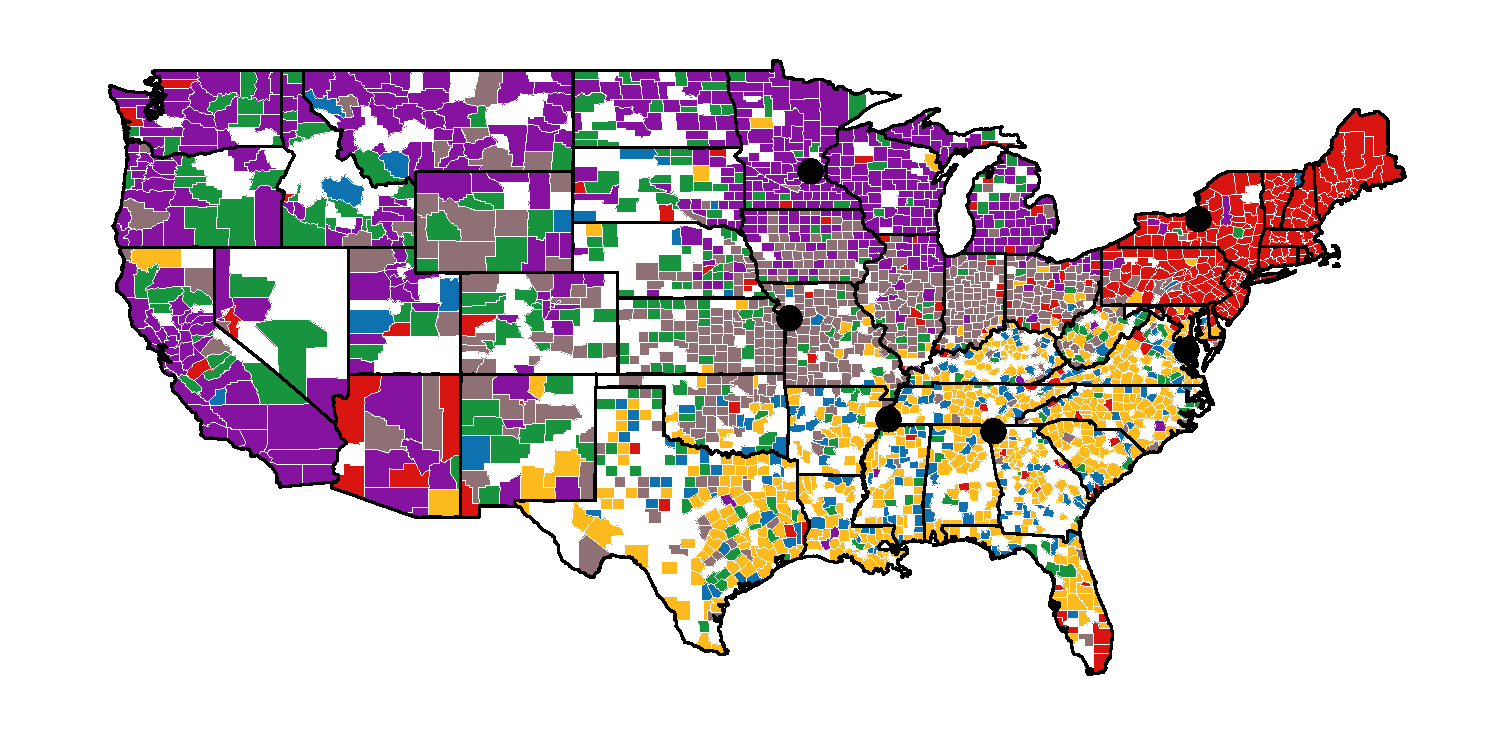
\includegraphics[width=1\textwidth]{fig/kmedoids6_raw.pdf}
        \caption{raw data with 6 clusters}
    \end{subfigure}
    \begin{subfigure}[t]{0.49\textwidth}
        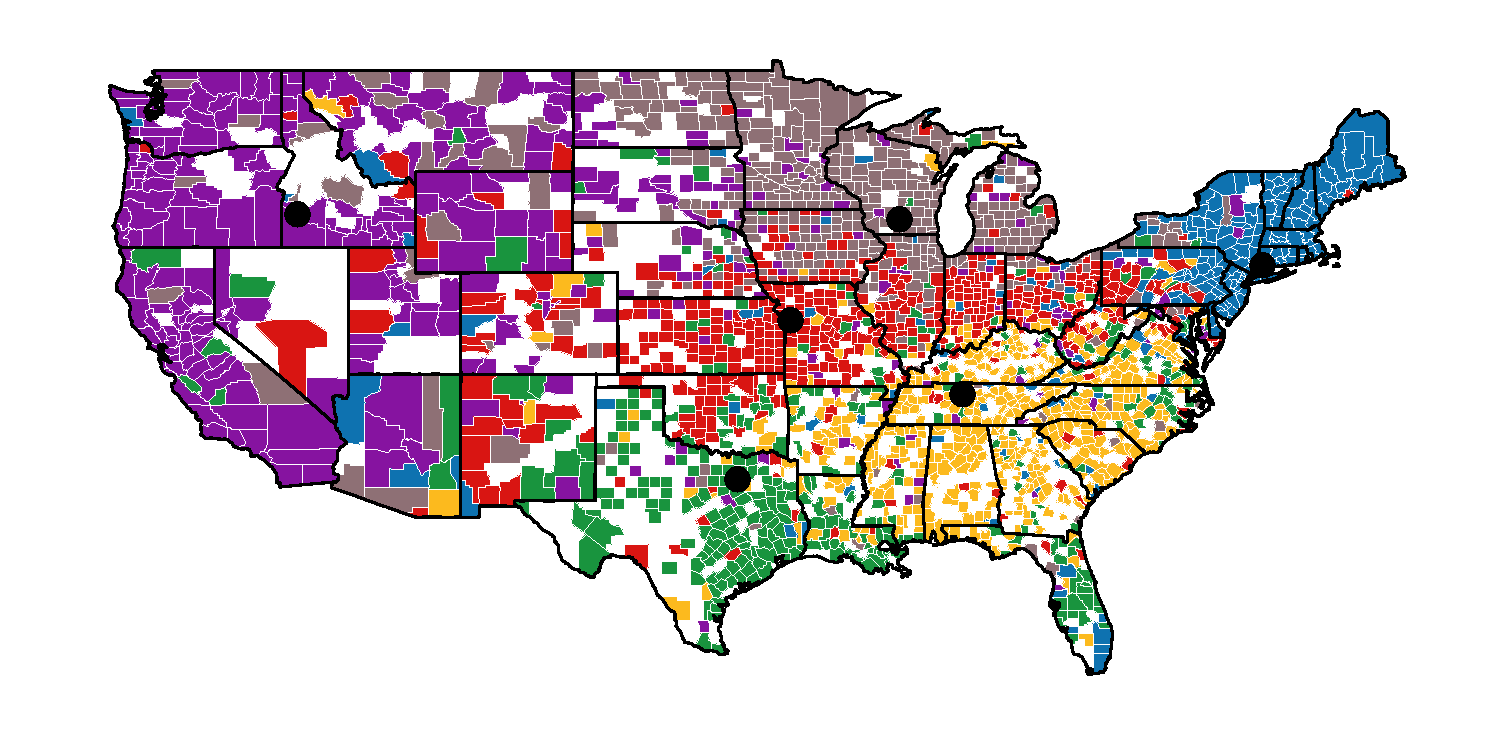
\includegraphics[width=1\textwidth]{fig/kmedoids6_PCA80.pdf}
                \caption{top 80 PCs with 6 clusters}
    \end{subfigure}
        \begin{subfigure}[t]{\textwidth}
        \centering
        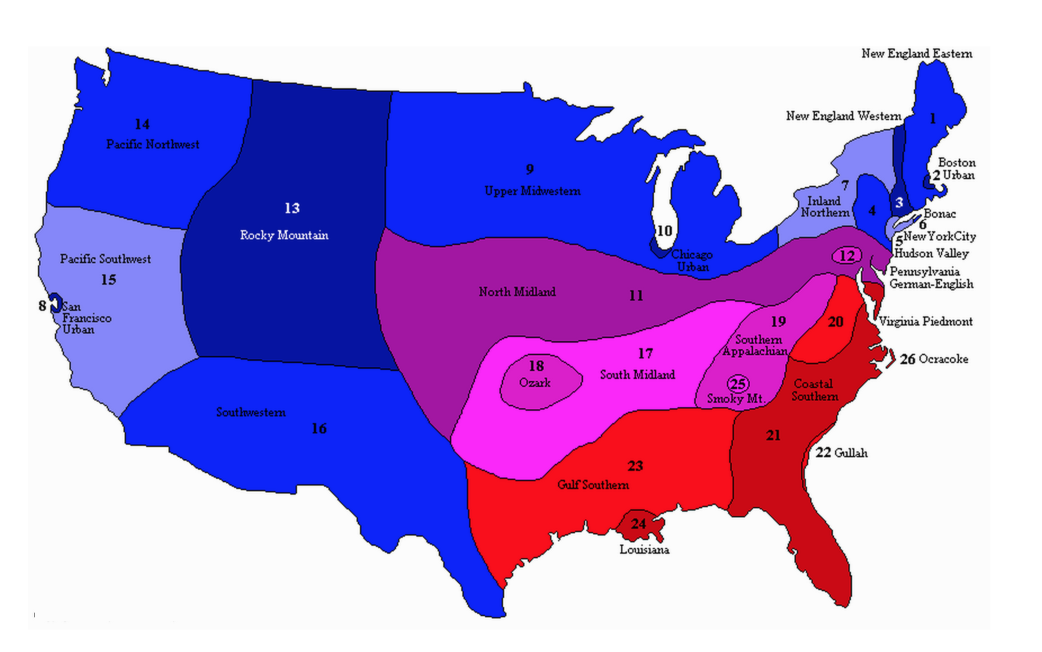
\includegraphics[width=0.6\textwidth, height= 0.4\textwidth]{fig/reference_map.pdf}
                \caption{Dialect Map of American English}
    \end{subfigure}
    \caption{\textbf{The clustering map for k-medoids when $k = 6$ on county level.} \textbf{(a)} Clustering based on the raw data with 6 clusters. \textbf{(b)}  Clustering based on the top 80 PCs with 6 clusters. The four black points are medoids. \textbf{(c)} \href{http://robertspage.com/dialects.html}{Dialect Map of American English} .} \label{fig: k-medoids_reference}
\end{figure}
